% Gerado exclusivamente de evidências locais; sem credenciais.
\newcommand{\DataRelatorio}{%
11 de novembro de 2026
}
\newcommand{\ResultadoAudio}{%
A avaliação foi regenerada com partições isoladas por família de frase-base. Os valores abaixo são extraídos de \path{evidence/audio_reproducao.json}; cada partição é reportada separadamente.
\begin{center}\begin{tabular}{lrrr}\toprule
Partição & Exemplos & Acurácia & F1 macro\\\midrule
Validação & 172 & 93,60\% & 0,933\\
Teste & 176 & 86,36\% & 0,862\\
Verificação cega & 120 & 88,33\% & 0,883\\
\bottomrule\end{tabular}\end{center}

}
\newcommand{\ResultadoNuvem}{%
Modelo utilizado: \textbf{gpt-4o-mini (texto) e gpt-4o-mini-transcribe (áudio)}. Chamadas reais registradas: \textbf{18}. Custo estimado acumulado: \textbf{US\$ 0,005980}. Estado registrado: 16 chamadas concluídas; duas respostas rejeitadas sem uso na decisão; inclui reserva conservadora da primeira falha.
}
\newcommand{\ResultadoTestes}{%
Suíte \textbf{pytest Python 3.12; entrega final}: 77 verificações aprovadas, 0 falhas.

Também foram aprovadas 26 verificações parametrizadas adicionais (subtestes), registradas separadamente da contagem de testes.
}
\newcommand{\ResultadoReplay}{%
Os registros completos da reprodução e da entrega estão em \path{integracao/evidencias/entrega_final_20261111/replay.json} e \path{integracao/evidencias/entrega_final_20261111/entrega_auditoria.json}.

No monitor incremental foram processados 32 pacotes. Latência local média: 0,631 ms; percentil 95 (posto mais próximo): 0,928 ms; máxima: 4,598 ms. O intervalo inclui detector estatístico, fusão e SQLite, conforme a instrumentação do monitor.
}
\newcommand{\ResultadoIntegracao}{%
Áudio novo-03, modelo congelado de treino, transcrição e análise textual reais do mesmo WAV, novo YOLO em montagem de teste e três fontes estruturadas sintéticas. Reserva por clipe apresentada separadamente, com seus eventos não detectados. No caso integrado, a confiança acústica do áudio novo-03 é 0,595, inferior ao limiar 0,70. A fonte de áudio fica inconclusiva e a cobertura permanece incompleta; o alerta alto do vídeo é preservado. Não se declara cobertura completa por terem sido fornecidos todos os arquivos.
}
\newcommand{\ResultadoRecursos}{%
GPU local NVIDIA RTX 2060: áudio anterior e novo YOLOv8s. Treino e inferência encerrados. Nenhuma sessão Colab foi iniciada. GPU utilizada nesta consolidação: sim. Sessão de computação encerrada ao final: sim.
}
\newcommand{\ResultadoMidias}{%
Foram criadas seis sínteses novas: duas referências e uma gravação reservada por voz. Não há hashes compartilhados com o corpus de 1.180 WAVs nem com as seis provas externas anteriores. O classificador emocional permaneceu congelado e não participou destes critérios.

\begin{center}\small\begin{tabular}{llcc}\toprule Voz & Cenário & Esperado & Obtido\\\midrule

Daniel & Original & Sem sinal & Sem sinal\\

Daniel & Volume reduzido & Sem sinal & Sem sinal\\

Daniel & Pausas inseridas & Sinal & Sinal\\

Daniel & Silêncio & Inconclusivo & Inconclusivo\\

Maria & Original & Sem sinal & Sem sinal\\

Maria & Volume reduzido & Sem sinal & Sem sinal\\

Maria & Pausas inseridas & Sinal & Sinal\\

Maria & Silêncio & Inconclusivo & Inconclusivo\\

\bottomrule\end{tabular}\end{center}

A versão interrompida insere 380 ms de silêncio a cada bloco de 180 ms. A versão com ganho reduzido multiplica a amplitude por 0,35. São perturbações técnicas, sem rótulo de doença; as derivações da mesma fonte não são observações independentes.

Dois vídeos geométricos novos passaram pelos cálculos reais de fluxo óptico: o controle não gerou eventos e o cenário alterado gerou 2. Não foi usado oráculo de caixas ou classes. Na montagem recebida foram processados 570 quadros e não houve aumento persistente que atingisse essa regra. Isso não significa ausência de eventos clínicos.

A reprodução contínua no ritmo original analisou 89 pares de quadros em 17,83 s de parede. Foram avaliadas 3 janelas de voz e persistidas 6 transições com sinais. O percentil 95 de processamento foi 15,20 ms por passo, além da espera da janela de cinco segundos. Não inclui ASR, nuvem ou captura clínica.

Evidência: \path{evidence/midias_complementares.json}. Nenhuma chamada paga foi feita nesta complementação.
}
\newcommand{\ResultadoVideoNovo}{%
A nova execução utilizou YOLOv8s, resolução de 416 por 416 pixels, batch 8, até 80 épocas e paciência 20. Foram concluídas 80 épocas, em 27,12 minutos de treinamento na GPU NVIDIA GeForce RTX 2060. A seleção usa somente a validação do primeiro prefixo de clipe.

\begin{center}\small\begin{tabular}{lrrr}\toprule Conjunto & Imagens & mAP50 & mAP50--95\\\midrule

Validação & 74 & 0,941 & 0,620\\

Teste & 37 & 0,980 & 0,615\\

Reserva de clipe & 60 & 0,613 & 0,299\\

\bottomrule\end{tabular}\end{center}

As métricas acima pertencem à nova execução e não são diretamente comparáveis ao mAP50 histórico: partições, preparação de anotações, batch e ambiente são diferentes. A queda de mAP50 do teste (mesmo prefixo do treino) para a reserva mostra que o valor alto no desenvolvimento não se mantém na outra origem disponível. Isso é compatível com diferenças de domínio e similaridade temporal, sem identificar uma causa única. A reserva não participou do treino, da escolha de limiares ou do checkpoint. O resultado entre prefixos não é validação em pacientes independentes.

Precisão e recall presentes no JSON são resumos de objetos da avaliação padrão Ultralytics. Não são os índices da regra temporal com limiares 0,4/0,6, cuja referência e resultados são registrados separadamente.

\begin{figure}[H]\centering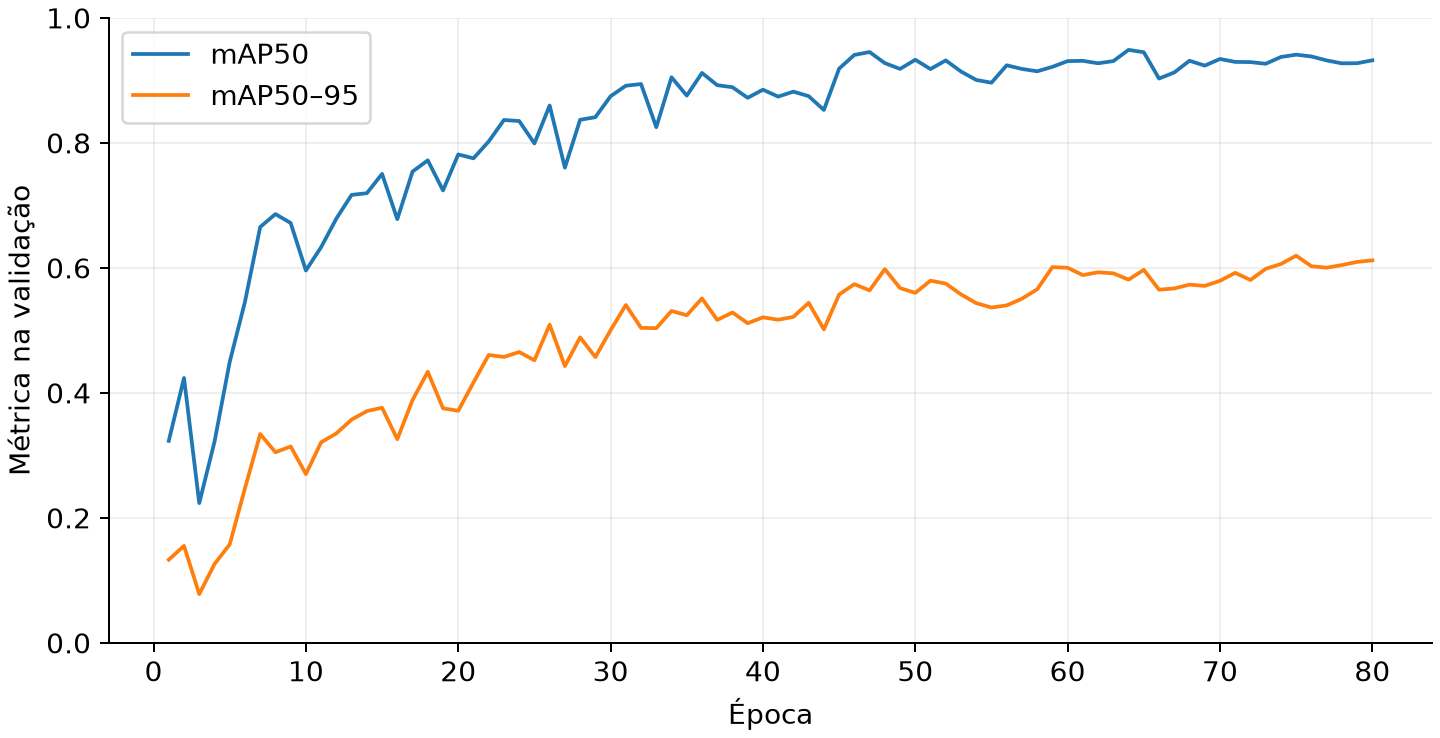
\includegraphics[width=0.92\textwidth]{figures/video_treino.png}\caption{Evolução da validação no novo treino YOLOv8s; a reserva de clipe não participa da curva.}\end{figure}

O peso congelado possui SHA-256 iniciado por \texttt{efe5cc2588300eea}. Evidências em \path{evidence/video_reproducao.json} e \path{evidence/video_dataset_auditoria.json}.

A montagem reservada foi construída após congelar o modelo, com 60 quadros-fonte não usados no desenvolvimento e duração de 120,0 segundos. A inferência gerou 0 evento(s). A referência temporal deriva das caixas anotadas e da própria regra de montagem; não é anotação clínica de complicações. A integração usa o teste para o exemplo positivo e mantém a reserva como verificação separada, sem ocultar seus eventos não detectados.

\begin{center}\small\begin{tabular}{lrrrr}\toprule Montagem & Referência & Sinalizados & Corretos & Não detectados\\\midrule

Teste & 3 & 2 & 2 & 1\\

Reserva & 2 & 0 & 0 & 2\\

\bottomrule\end{tabular}\end{center}

Os eventos são pareados uma única vez com IoU temporal de pelo menos 0,5. No teste, dois de três eventos foram recuperados (precisão 1,00 e recall 0,667). Na reserva, os dois eventos de referência não foram detectados: recall 0 e precisão não definida, pois não houve previsão positiva. A avaliação evidencia uma limitação de generalização da regra com o novo detector. Os limiares não foram ajustados depois de observar essa reserva.
}
\newcommand{\ComandosReproducao}{%
\begin{enumerate}
\item Preparar Python e instalar as dependências descritas no README.
\item Executar \code{python -m pytest -q} para a suíte de software.
\item Executar \code{python scripts/run_demo.py --help} para conferir entradas e diretório de saída.
\item Informar o CSV regenerado, o JSON de vídeo e o resultado textual real ao script de demonstração.
\item Abrir o painel com \code{python -m techchallenge4.dashboard --help} e selecionar o banco gerado.
\item Compilar o relatório com \code{python relatorio/gerar_relatorio.py --compile --package} ou importar o ZIP no Overleaf.
\end{enumerate}
}
\newcommand{\ManifestoEvidencias}{%
\small\begin{longtable}{p{8.7cm}p{4.4cm}}\toprule
Artefato & SHA-256 (prefixo)\\\midrule\endhead
\path{evidence/video_dataset_auditoria.json} & \texttt{8f14126d114c5190}\\
\path{evidence/video_reproducao.json} & \texttt{e267cdb305d3734d}\\
\path{evidence/video_inferencia_nova.json} & \texttt{30b88d7ec6fc141a}\\
\path{artifacts/video/manifesto_video.json} & \texttt{ca6187addfca1461}\\
\path{evidence/midias_complementares.json} & \texttt{4a1ad23c210416af}\\
\path{evidence/padrao_relatorio.json} & \texttt{dce7f0f2b99dd414}\\
\path{evidence/audio_reproducao.json} & \texttt{eec78c6135392737}\\
\path{audio/evidencias/particoes_audio.csv} & \texttt{30dc41d77d9167b3}\\
\path{audio/evidencias/predicoes_avaliacao.csv} & \texttt{a6b46c44b1312d97}\\
\path{artifacts/audio/manifesto_audio.json} & \texttt{fafd4dbbe961e037}\\
\path{evidence/resumo_execucao.json} & \texttt{7c9db7bb48fd5af2}\\
\path{evidence/audio_externo_transcricoes.json} & \texttt{8da6101b626df962}\\
\path{evidence/asr_comparacao.json} & \texttt{c86c4ff64c6c6263}\\
\path{evidence/audio_externo.json} & \texttt{20d055c33a303003}\\
\path{evidence/audio_recebido_drive.json} & \texttt{99a156e55c61acef}\\
\path{evidence/openai_validacao.json} & \texttt{9e43f13d89c3dc42}\\
\path{evidence/video_validacao.json} & \texttt{17832e5417cf354e}\\
\path{evidence/dashboard_validacao.json} & \texttt{e994518026d1aa81}\\
\path{integracao/evidencias/monitoramento_final/monitoramento_resumo.json} & \texttt{20c95ef1eec67a2b}\\
\path{integracao/evidencias/entrega_final_20261111/replay.json} & \texttt{8d1fc82c0db89420}\\
\path{integracao/evidencias/entrega_final_20261111/entrega_auditoria.json} & \texttt{70822b703e34beeb}\\
\path{integracao/evidencias/entrega_final_20261111/anomalias_estruturadas.json} & \texttt{e5e6f55892ed79b8}\\
\bottomrule\end{longtable}\normalsize
Os hashes completos devem ser consultados nos manifestos de execução e no histórico do repositório. O prefixo serve como referência de leitura, não como substituto de uma verificação integral.
}
